\documentclass[a4paper, 10pt]{article}
\usepackage{graphicx}
\usepackage{float}
\usepackage{geometry}
\usepackage[font=small, skip=0pt]{caption}
\usepackage{subcaption}
\usepackage{siunitx}
\usepackage{fancyhdr}
\geometry{margin=20mm}
\setlength{\textfloatsep}{4pt plus 1.0pt minus 2.0pt}
\setlength{\intextsep}{6.0pt plus 1.0pt minus 1.0pt}
\setlength{\belowcaptionskip}{-6pt}

\pagestyle{fancy}
\lhead{COMS30127 Lab 2}

\begin{document}

\section*{COMS30127 Lab 2: Model of a Single Neuron}

\subsection*{Part 1: Simulated Integrate and Fire Model Neuron}
\begin{figure}[H]
  \centering
  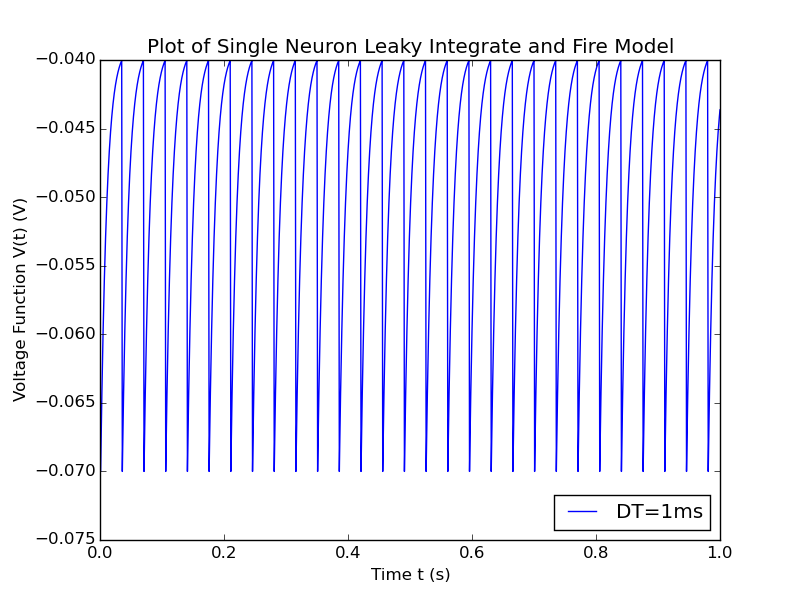
\includegraphics[scale=0.4]{p1.png}
  \caption{The voltage of a single neuron with fixed input current simulated with the integrate and fire model for \SI{1}{\second}.}
  \label{fig:n1}
\end{figure}

\subsection*{Part 2: Minimum Current for Action Potential}

The minimum required current, \(I_{min}\), for an action potential is \SI{3}{\nano\ampere}.

\begin{figure}[H]
  \centering
  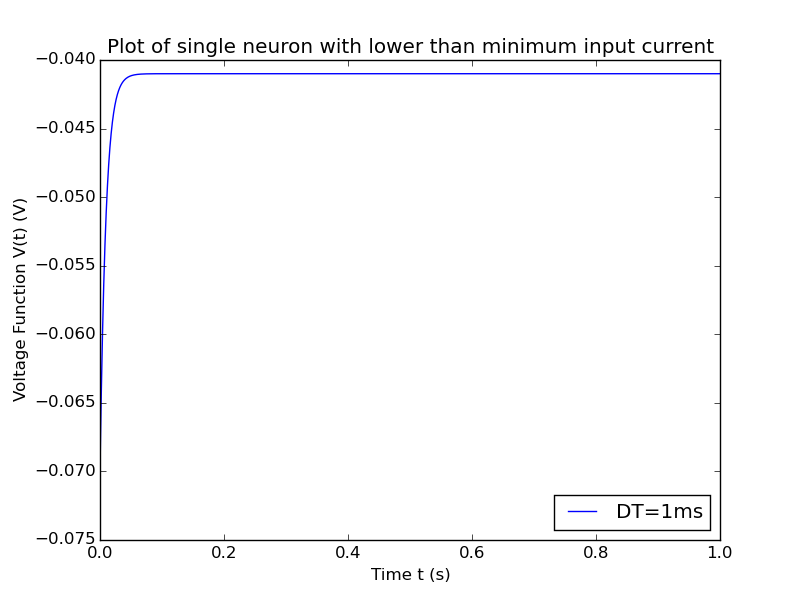
\includegraphics[scale=0.4]{p2b.png}
  \caption{Simulation of the neuron from Part 1 with the fixed input current reduced to \(I_{min} - \SI{0.1}{\nano\ampere}\).}
\end{figure}

\subsection*{Part 3: Simulated Firing Rate Against Input Current}

\begin{figure}[H]
  \centering
  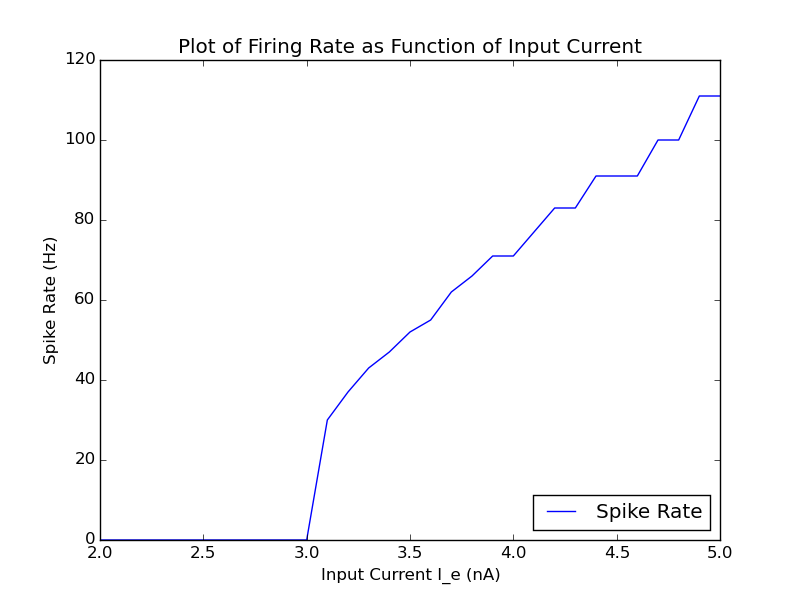
\includegraphics[scale=0.4]{p3.png}
  \caption{The firing rate for fixed input currents ranging from \SI{2}{\nano\ampere} and \SI{5}{\nano\ampere} sampled at \SI{0.1}{\nano\ampere} intervals, from \SI{1.0}{\second} simulations.}
\end{figure}

\subsection*{Part 4: Neuron Pair with Synaptic Connections}
\begin{figure}[H]
  \centering
  \begin{subfigure}{.5\textwidth}
    \centering
    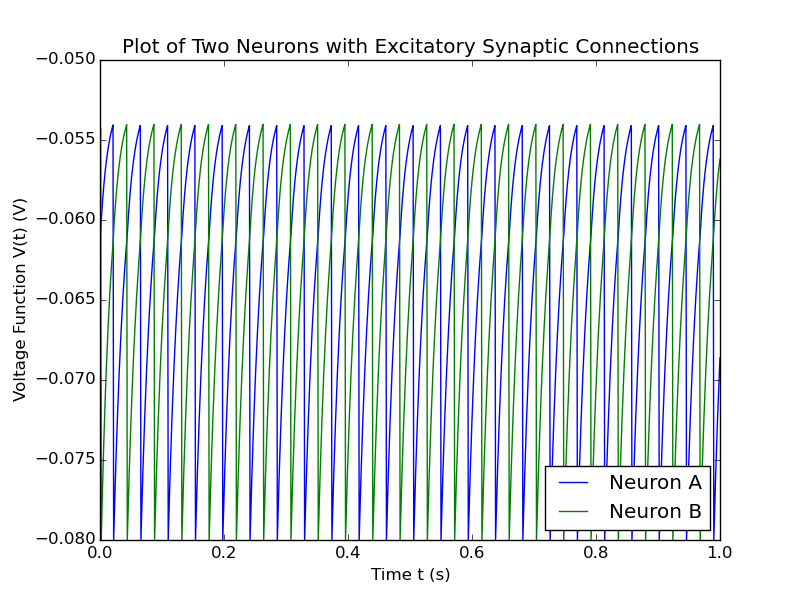
\includegraphics[scale=0.4]{p4_Excitatory.png}
    \caption{Excitatory Synaptic Connection}
    \label{fig:sub1}
  \end{subfigure}%
  \begin{subfigure}{.5\textwidth}
    \centering
    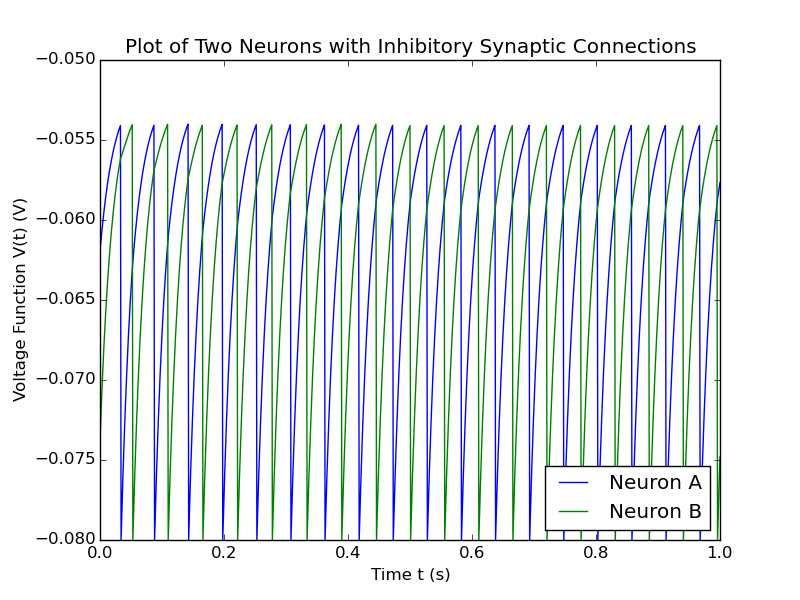
\includegraphics[scale=0.4]{p4_Inhibitory.png}
    \caption{Inhibitory Synaptic Connection}
    \label{fig:sub2}
  \end{subfigure}
  \par\medskip
  \caption{Plot of the voltage of two neurons with synaptic connections of differing types over time.}
\end{figure}

\vspace{5mm}
The excitatory synaptic connection plot in figure \ref{fig:sub1} shows that the time between spikes quickly converges. This is because when one neuron spikes, the post-synaptic neuron experiences an increase of voltage. Converseley, the inhibitory synaptic connection in figure \ref{fig:sub2} shows that the spiking frequencies become out of phase. This is due to the post-synaptic potential decreasing. In both cases, the effect is compounded as the neurons spike, causing the effect to become more pronounced (until the neurons are either completely in or out of phase, respectively.

\subsection*{Part 5: Slow Potassium Current}
\begin{figure}[H]
  \centering
  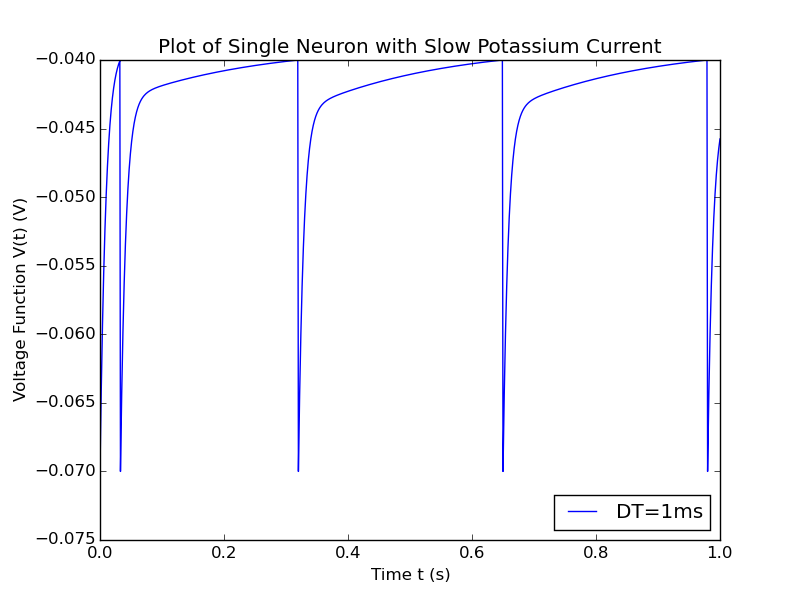
\includegraphics[scale=0.4]{p5.png}
  \caption{The simulated neuron shown in figure \ref{fig:n1} with an added slow potassium current.}
\end{figure}

\end{document}
